% This is samplepaper.tex, a sample chapter demonstrating the
% LLNCS macro package for Springer Computer Science proceedings;
% Version 2.20 of 2017/10/04
%
\documentclass[runningheads]{llncs}
% 
\usepackage{graphicx}
\usepackage{listings}
% Used for displaying a sample figure. If possible, figure files should
% be included in EPS format.
%
% If you use the hyperref package, please uncomment the following line
% to display URLs in blue roman font according to Springer's eBook style:
% \renewcommand\UrlFont{\color{blue}\rmfamily}
\usepackage{lettrine} % Pacote para formatação especial da primeira letra
\usepackage{hyperref}
\begin{document}
%
\title{Correlating Obesity and Mental Illnesses}
% Coloca o DOI aqui se o artigo já tiver sido publicado; caso contrário, deixa como "To be assigned"
\titlerunning{DOI: To be assigned}
% If the paper title is too long for the running head, you can set
% an abbreviated paper title here
%
\author{Diogo Esteves\inst{1} \and Rui Sousa\inst{2}}
%
\authorrunning{Esteves, D. and Sousa, R.}
% First names are abbreviated in the running head.
% If there are more than two authors, 'et al.' is used.
%
\institute{Department of Informatics, University of Minho, Portugal\\
\email{pg28935@alunos.uminho.pt\inst{1} pg21019@alunos.uminho.pt}\inst{2}\\
\url{http://www.di.uminho.pt}}

\maketitle 
\begin{abstract}
The prevalence of obesity and mental health disorders has reached unprecedented levels globally, presenting significant challenges to public health systems. This study delves into the intricate relationship between obesity, mental illness, and socioeconomic factors, utilizing comprehensive datasets from \href{https://ourworldindata.org/}{Our World in Data}. Through a multidimensional analysis, we investigate the bidirectional association between obesity and mental health disorders, exploring how socioeconomic status influences this complex interplay.

Our findings reveal a consistent rise in the prevalence of obesity, depression, anxiety, bipolar disorder, and schizophrenia, paralleling population growth trends. Notably, lower socioeconomic status emerges as a significant determinant, exacerbating both obesity and mental health disorders through various pathways, including limited access to healthy foods and increased stress levels.

Moreover, our study underscores the importance of integrated healthcare strategies that address the holistic needs of individuals, considering both physical and mental well-being.

\keywords{Poverty \and Obesity \and Mental \and Illness \and Socioeconomic Factors \and Data Analysis \and Health Disparities \and Nutritional Economics \and Psycho-social Stress}
\end{abstract}
%
%
%
\section{Introduction}
Obesity rates around the developed world are unprecedented, representing one of the most rapidly observed phenotype alterations in human populations in developed countries \cite{Bentley2018}. Despite food access being universally recognized as a fundamental human necessity, the quality and nutritional value of available food sources exert a profound influence on individual health outcomes. With the proliferation of industrially processed foods, there has been an emergence of abundant, highly caloric, and cost-effective food options. This dietary pattern may not only contribute to but also exacerbate a myriad of health problems due to its potential impact on the body, including but not limited to reduction in gut microbiome diversity, diabetes, and cardiovascular diseases \cite{Bentley2018,Smits2017,Muscogiuri2018}.

Beyond physical health, the repercussions of poor dietary habits extend to mental well-being. A growing body of evidence suggests a bidirectional relationship between obesity and mental illness, with each condition mutually influencing and worsening the other. As individuals navigate the challenges posed by poverty, the stressors associated with financial instability and limited resources often compound existing mental health vulnerabilities, predisposing them to conditions such as depression and anxiety \cite{Zhang2021}.

In light of these considerations, this study seeks to affirm the interplay between obesity and mental illness through a thorough analysis of prevalence data across diverse socioeconomic strata. Specifically, our aim is to ascertain whether a correlation exists whereby obesity and mental disorders exhibit a bidirectional relationship. This exploration will involve an extensive review of current literature, analysis of epidemiological data, and examination of underlying mechanisms that might explain the observed trends.

\subsection{Obesity and Mental Health}
The association between obesity and mental health disorders is increasingly recognized as a significant public health issue. Obesity has been linked to a higher prevalence of mental health conditions such as depression, anxiety, and eating disorders \cite{Luppino2010}. The relationship between obesity and mental health is complex and bidirectional; mental health issues can lead to changes in eating behaviors and physical activity, which can contribute to weight gain, while obesity can, in turn, affect mental well-being.

Depression is one of the most common mental health disorders associated with obesity. Several studies have demonstrated that individuals with obesity are at a higher risk of developing depression and vice versa \cite{Faith2011}. The mechanisms underlying this association are not fully understood but may involve biological, psychological, and social factors. For instance, obesity-related inflammation has been suggested to play a role in the pathophysiology of depression \cite{Berk2013}.

Anxiety disorders, including generalized anxiety disorder, panic disorder, and social anxiety disorder, have also been linked to obesity. The relationship between anxiety and obesity may be mediated by various factors, including stress-related eating, poor body image, and social stigma associated with being overweight or obese \cite{Scott2008}.

\subsection{Socioeconomic Factors and Obesity}
Socioeconomic status (SES) is a significant determinant of obesity, with lower SES being associated with higher rates of obesity. This relationship is influenced by various factors, including access to healthy food, opportunities for physical activity, and health literacy. Individuals from lower socioeconomic backgrounds often face barriers to accessing nutritious foods, such as living in food deserts where healthy food options are scarce and expensive \cite{Drewnowski2004}.

Moreover, lower SES is often associated with higher levels of stress due to financial instability, job insecurity, and limited access to healthcare. Chronic stress can lead to behaviors that contribute to weight gain, such as overeating, consumption of high-calorie foods, and reduced physical activity \cite{Goodman2003}. Additionally, stress activates the hypothalamic-pituitary-adrenal (HPA) axis, leading to increased secretion of cortisol, a hormone that promotes fat storage, particularly in the abdominal area \cite{Charmandari2005}.

\subsection{Obesity, Mental Health, and Socioeconomic Status: An Integrated Perspective}
The interplay between obesity, mental health, and socioeconomic status is complex and multifaceted. Lower socioeconomic status not only predisposes individuals to obesity but also to mental health disorders. The stressors associated with financial instability, lack of social support, and limited access to mental health services can exacerbate both obesity and mental health issues \cite{Everson2002}.

Furthermore, there is evidence to suggest that the relationship between obesity and mental health is moderated by socioeconomic factors. For instance, the stigma associated with obesity may be more pronounced in higher socioeconomic groups, where there is greater emphasis on physical appearance and health, potentially leading to greater psychological distress among obese individuals in these groups \cite{Puhl2009}.

Conversely, individuals from lower socioeconomic backgrounds may experience a different set of challenges. The lack of resources and opportunities for healthy living can lead to a cycle of poor physical and mental health outcomes. For example, food insecurity, a common issue among low-income families, is associated not only with higher rates of obesity but also with increased rates of depression and anxiety \cite{Laraia2013}.

\section{Methods}

The datasets utilized in this research project are sourced from the \href{https://ourworldindata.org/}{Our World in Data repository}. We have selected distinct datasets that examine the incidence and prevalence of mental diseases, obesity, education levels, and poverty over time.

The obesity dataset examines a wide range of characteristics associated with obesity and its correlations, including mortality rates, risk of coronary diseases, and gender-specific prevalence. For the purposes of this study, we will focus on the percentage of adults who are overweight or obese and the overall prevalence of obesity in adults \cite{Obesity}.

The dataset on mental illnesses, like the previously mentioned datasets, examines the prevalence, burden of disease, and risk factors of various mental illnesses worldwide. Our focus will be exclusively on the prevalence of mental disorders, specifically depression, bipolar disorder, anxiety disorder, and schizophrenia. Additionally, we will attempt to link the eating disorder data within this dataset to the obesity statistics\cite{MentalHealth}.

The data was preprocessed and analysed using standard statistical treaments, using Python Pandas and PowerBI to handle most of the operations: cleaning, filtering, slicing and correlating. 

\section{Results}
The data for all countries reveals a consistent and discernible rise in the prevalence of several illnesses over time, including eating disorders, obesity, depression, anxiety, bipolar disorder, and schizophrenia. Interestingly, there appears to be a proportional relationship between this trend and the overall population growth. For instance, both obesity and eating disorders show an upward trajectory in tandem with population expansion, indicating a correlation between these health issues and population growth \cite{jeatdisord2019,cambridge2020}.

\begin{figure}[ht!]
    \centering
    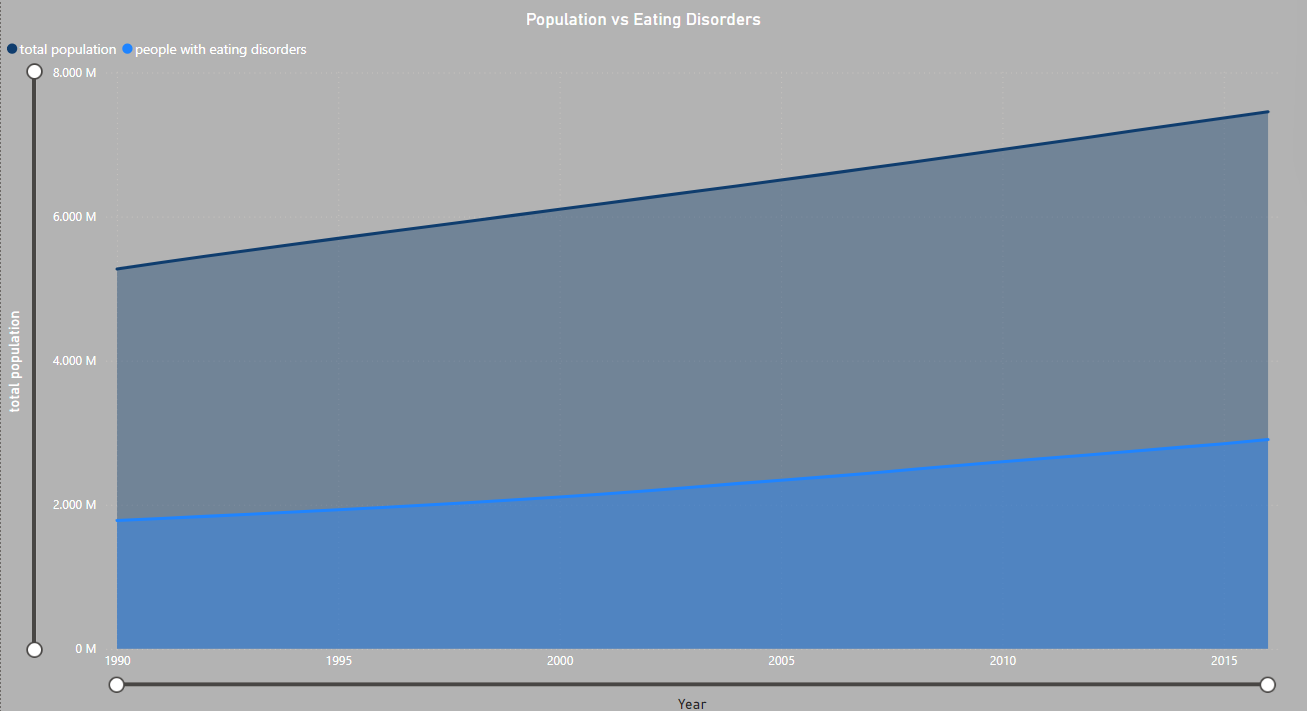
\includegraphics[width=\textwidth]{./imgs/Eating disorders.png}
    \caption{Population vs Eating Disorders}
    \label{fig:eatingdisorders}
\end{figure}

\clearpage

\begin{figure}[ht!]
    \centering
    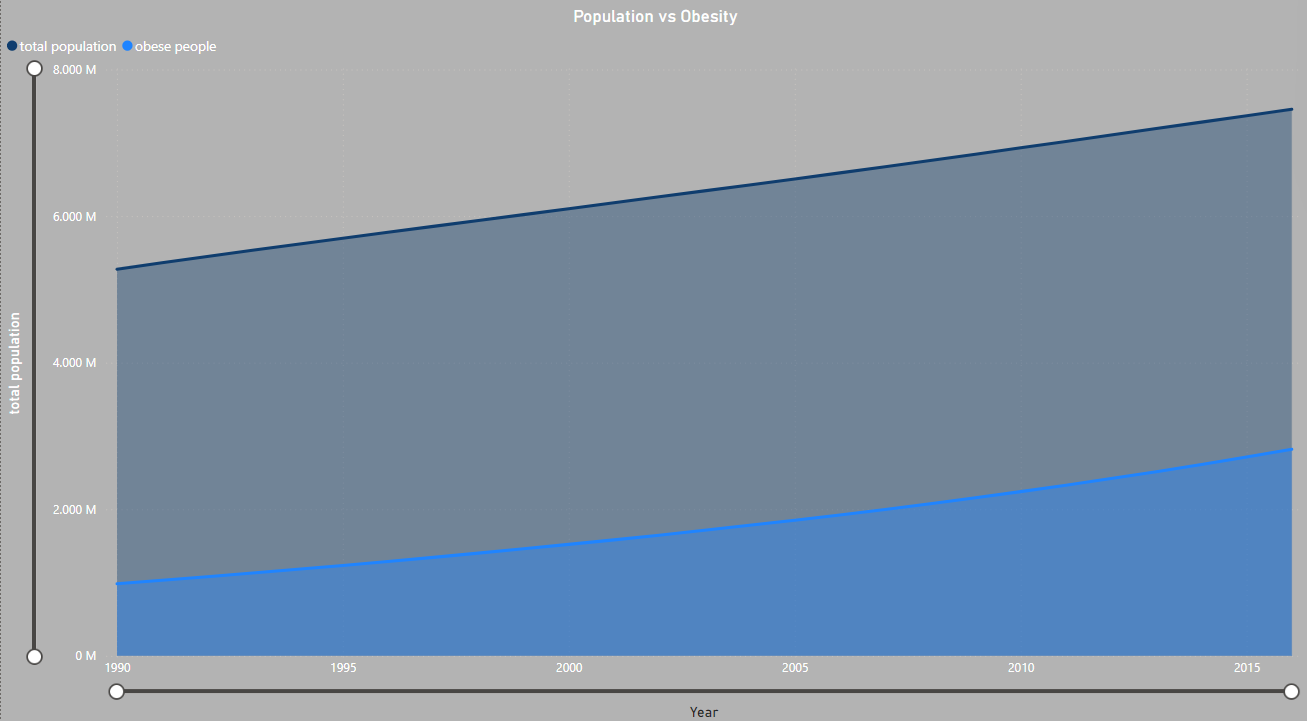
\includegraphics[width=\textwidth]{./imgs/obes.png}
    \caption{Population vs Obesity}
    \label{fig:obesity}
\end{figure}

Anxiety and depression also exhibit consistent increases, supporting the idea that population dynamics and mental health diseases are strongly related \cite{bmjpsychiatry2020}.

\begin{figure}[ht!]
    \centering
    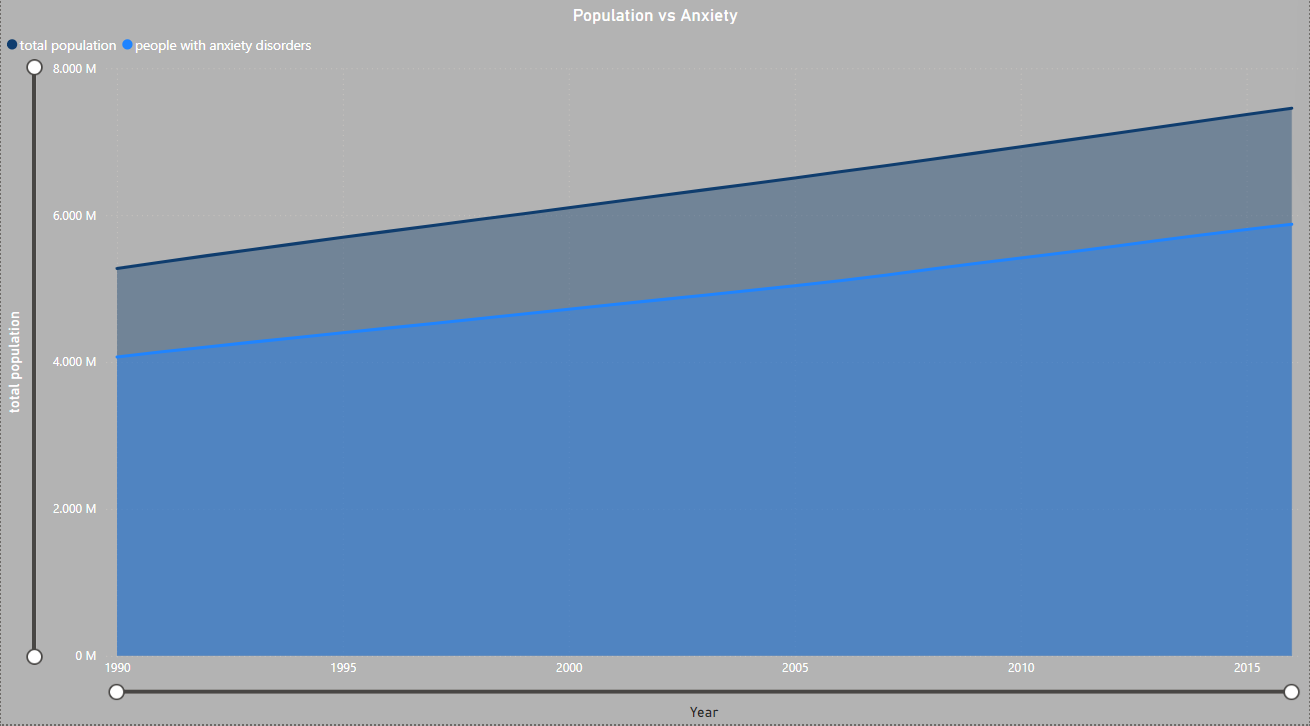
\includegraphics[width=\textwidth]{./imgs/anxiety.png}
    \caption{Population vs Anxiety}
    \label{fig:anxiety}
\end{figure}

\begin{figure}[ht!]
    \centering
    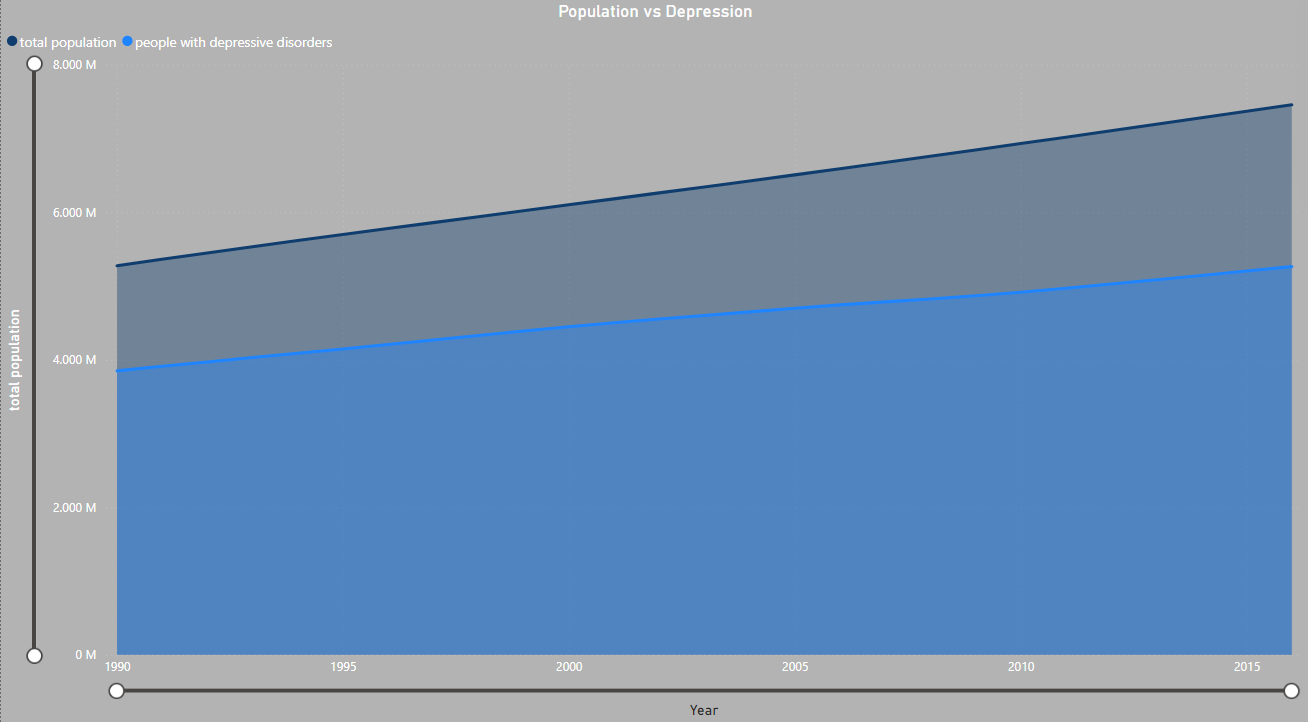
\includegraphics[width=\textwidth]{./imgs/depress.png}
    \caption{Population vs Depression}
    \label{fig:depress}
\end{figure}

Further analysis of bipolar disorder and schizophrenia also supports this trend, with both disorders exhibiting a significant and proportional increase relative to population growth. 

\begin{figure}[ht!]
    \centering
    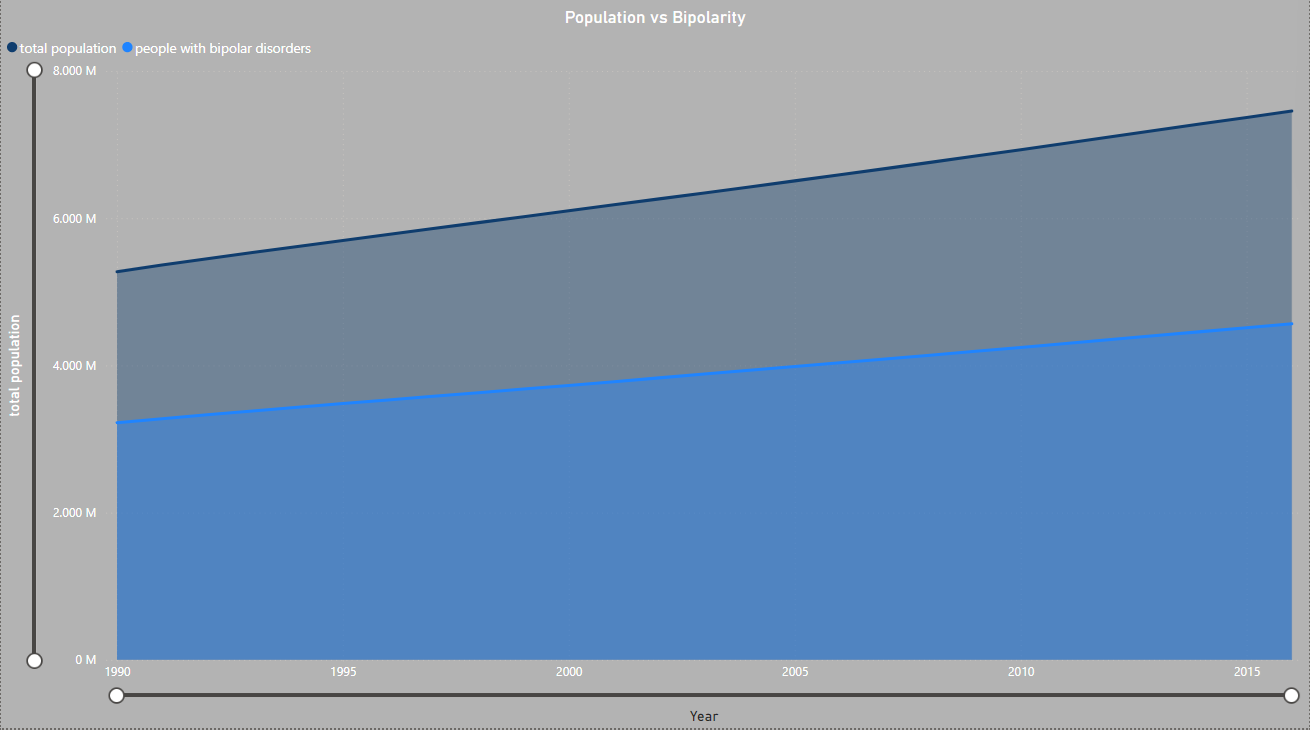
\includegraphics[width=\textwidth]{./imgs/bipolar.png}
    \caption{Population vs Bipolar Disorder}
    \label{fig:bipolar}
\end{figure}

\begin{figure}[ht!]
    \centering
    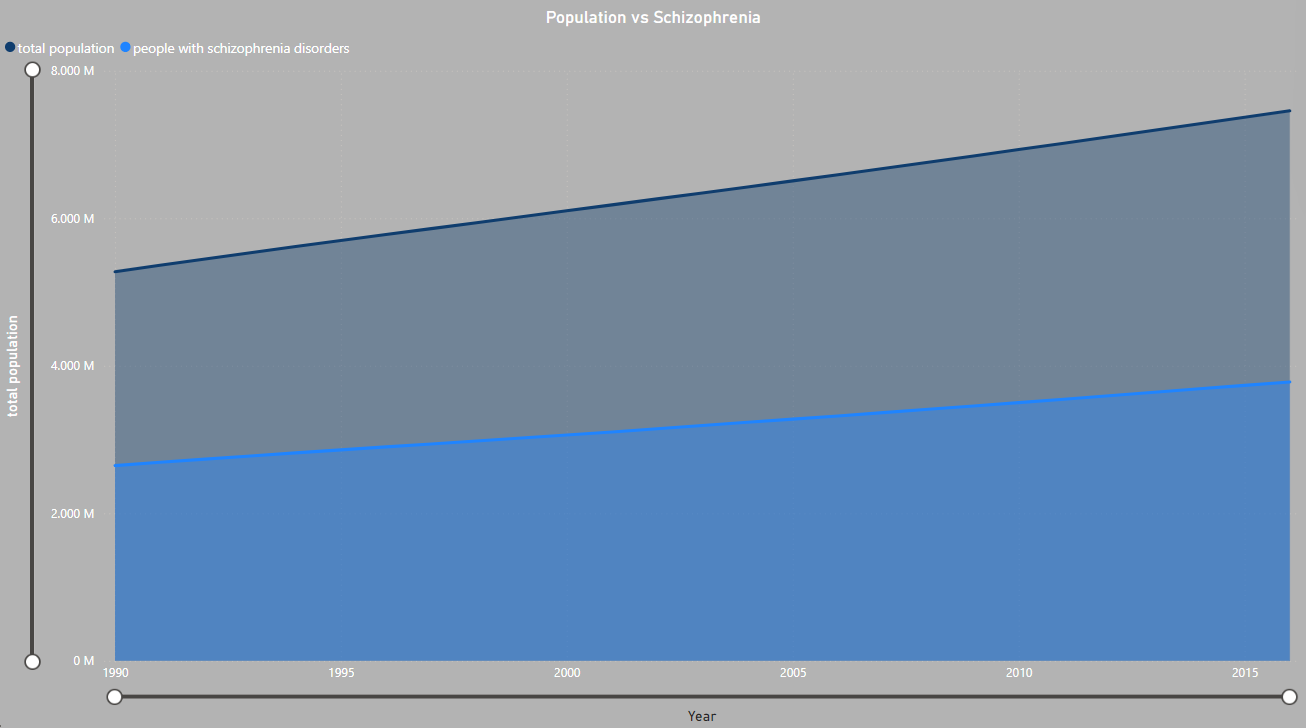
\includegraphics[width=\textwidth]{./imgs/schizo.png}
    \caption{Population vs Schizophrenia}
    \label{fig:schizo}
\end{figure}

The consistent pattern observed across these disorders implies that various factors associated with an increasing population—such as social, economic, and environmental changes—may contribute to the rising prevalence of these conditions \cite{jeatdisord2019}. This correlation underscores the importance of addressing underlying causes and implementing public health strategies to manage and mitigate the impact of these disorders.

In conclusion, the analysis highlights a significant finding in the field of public health: a direct correlation exists between population growth and the prevalence of eating disorders and mental health issues. This trend suggests that the prevalence of these conditions will increase alongside population growth. Therefore, policymakers, healthcare professionals, and researchers must consider the broader implications of population dynamics when developing interventions and policies to mitigate the occurrence and impact of these health conditions. Further exploration and in-depth analysis within the provided Power BI file can yield additional insights and guide more targeted efforts to improve public health outcomes \cite{jeatdisord2019,cambridge2020,bmjpsychiatry2020}.

\section{Conclusions}

In this study, we investigated the complex relationship between obesity and mental disorders, utilizing extensive datasets from the Our World in Data repository. Our analysis confirmed a significant correlation between obesity and mental disorders, corroborating the bidirectional relationship described in the literature. This means that not only can obesity contribute to the onset of mental health issues, but mental health problems can also lead to obesity. This complex interplay underscores the need for integrated healthcare approaches that address both physical and mental health simultaneously.

The data also highlighted that the prevalence of obesity is particularly severe in the United States. This finding aligns with existing research, which points to lifestyle, dietary habits, and socio-cultural factors prevalent in the United States as significant contributors to the high rates of obesity. Factors such as the widespread availability of high-calorie, processed foods and a sedentary lifestyle are well-documented contributors to this public health issue.

Our study primarily focused on the correlation between obesity and mental health, but it also opens avenues for future research. One critical area for further investigation is the impact of socio-economic conditions and literacy on obesity. The literature suggests that socio-economic status plays a pivotal role in obesity rates due to disparities in access to nutrient-rich foods and varying levels of nutritional knowledge. Lower-income individuals often have limited access to healthy food options and may lack the education necessary to make informed dietary choices, leading to higher obesity rates.

Future research could benefit from analyzing datasets that include variables such as income levels, educational attainment, and food availability to better understand these socio-economic impacts. For instance, examining the correlation between education levels and obesity could reveal how nutritional literacy influences dietary choices and health outcomes. Additionally, understanding the role of socio-economic status could inform public health interventions aimed at reducing obesity by improving access to healthy foods and increasing nutritional education, particularly in underserved communities.

Furthermore, investigating the effects of socio-economic conditions on mental health could provide a more holistic understanding of the interplay between obesity, mental health, and socio-economic factors. Financial instability, for instance, is a known stressor that can exacerbate mental health issues, which in turn may lead to unhealthy eating habits and obesity. By examining these variables together, researchers can develop more comprehensive strategies to tackle obesity and mental health issues concurrently.

In conclusion, our findings emphasize the need for integrated public health strategies that address both physical and mental health, particularly in regions with high obesity prevalence like the United States. Future research should explore the socio-economic determinants of obesity to develop targeted interventions that address the root causes of this complex issue. By focusing on improving nutritional literacy and access to healthy foods, especially in low-income populations, we can work towards reducing obesity rates and improving overall health outcomes. This holistic approach is essential for effectively combating the intertwined epidemics of obesity and mental health disorders.



%
% ---- Bibliography ----
%
% BibTeX users should specify bibliography style 'splncs04'.
% References will then be sorted and formatted in the correct style.
%
%\bibliographystyle{splncs04}
\bibliographystyle{unsrt}
\bibliography{bibliography}
%

\end{document}